\addchap{Flüchtlinge in Dresden}

Wenn du aus Dresden kommst, wirst du es bereits mitbekommen haben, aber für alle, die neu in unserer Stadt sind: Wie eine Vielzahl anderer Städte in Deutschland (und ganz Europa), ist auch Dresden mit seinen 500.000 Einwohnern Anlaufpunkt für viele geflüchtete Menschen geworden. Die aktuelle politische Lage in Europa und die sächsische Flüchtlingspolitik stellen dabei die Stadt, unzählige freiwillige Helfer, offizielle Hilfsorganisationen wie das DRK, und letztendlich unsere ganze Gesellschaft vor eine große Herausforderung. 

Die meisten der geflüchteten Menschen sind mit ihrer Ankunft in Deutschland und Dresden dem Krieg und der Verfolgung in ihrem Heimatland entkommen und nach teilweise mehrjähriger Flucht nun hier in Sicherheit. In Dresden gibt es mehrere Erstaufnahmestellen, die hunderten Flüchtlingen eine vorläufige Unterkunft bietet, bis ihnen eine dezentrale Unterkunft in oder um Dresden vermittelt wird. Eine stellt die Zeltstadt an der Bremer Straße in Dresden Friedrichstadt dar, in der über 1.000 Menschen untergebracht sind.

Auch in den Sportstätten an der Nöthnitzer Straße direkt neben dem APB ist im August diesen Jahres eine Erstaufnahmestelle für mehr als 600 Menschen, darunter etwa 90 Kinder, eingerichtet worden. \link{http://www.dnn-online.de/dresden/web/dresden-nachrichten/detail/-/specific/Ab-Montag-sollen-rund-600-Asylsuchende-in-Dresdner-TU-Turnhallen-untergebracht-werden-571191965}  Beide Unterkünfte werden vom DRK betreut.

Die Umnutzung der Hallen hat für uns Studierende den Nebeneffekt, dass kommendes Semester in diesen Hallen keine Sportangebote stattfinden werden können. Nach Ausweichlösungen wird aktuell gesucht. Alle Infos dazu findest du auf den Seiten des USZ \link{https://tu-dresden.de/usz} und auch das Rektorat informiert regelmäßig über Neuigkeiten und Änderungen, die die Unterbringung an der Nöthnitzerstraße betreffen. 

Außerdem wurden die Schließzeiten des APB verändert. Bisher war die Fakultät immer offen, jetzt ist das nur noch Montag bis Freitag von 6 bis 19 Uhr der Fall. Das heißt aber nicht, dass du zu den anderen Zeiten nicht rein oder raus kommt. An der rechten inneren Tür befindet sich eine Klingel, gegen Vorzeigen des Studentenausweises lässt dich der Wachmann jederzeit rein, und raus kommt man sowieso immer.

Ohne das ehrenamtliche Engagement vieler Bürger Dresdens und vieler Studierender wäre die Unterbringung der bisher über 1.200 Geflüchteten, die dieses Jahr neu in Dresden angekommen sind, nicht möglich gewesen. Momentan leben mehr als 2.600 Asylsuchende in Dresden und es werden bis Ende des Jahres noch gut 2.000 weitere Neuankömmlinge erwartet. \link{https://www.dresden.de/media/pdf/sozialamt/Zahlen-und-Prognosen-Asyl.pdf} (Zahlen vom 31.7.2015) 

Nach wie vor ist viel Arbeit zu tun, da auch weiterhin Flüchtlinge nach Dresden kommen werden, und die Hilfsorganisationen leider überfordert sind. Es gibt in Dresden sehr viele Initiativen und Gruppen, die sich für Flüchtlinge, Asylsuchende und Migranten einsetzen. 

Wenn du selber mithelfen willst, wendest du dich am besten an das im April 2015 gegründete Netzwerk \textit{Dresden für Alle} \link{https://www.facebook.com/dresdenfueralle}. In diesem sind über 80 Vereine und Organisationen Dresdens vertreten. Außerdem gibt es in vielen Stadtteilen Willkommensbündnisse, die stets freiwillige Helfer suchen.

Weiterhin bietet die interaktive Vernetzungsplattform \textit{Afeefa} \link{http://afeefa.de} einen Überblick über die Initiativen der Stadt. Auch direkt an der Uni kannst du dich als Helfer melden und z.B. im USZ beim DRK mitwirken. Dazu schreibe an \textit{mithilfe@tu-dresden.de} folgende Informationen:

Name, Vorname, Geburtsdatum, ab wann einsetzbar, für wie lange einsetzbar, welche Qualifikationen und speziellen Fähigkeiten, Mailadresse, Telefon- oder Handynummer, Sprachen, Einwilligung zur Weitergabe dieser Angaben ans DRK.

Außerdem existiert zur Koordination der studentischen Hilfe in der Einrichtung im USZ eine Facebookgruppe \link{https://www.facebook.com/groups/helferfureaedd2}.

\vfill

\begin{figure}[h!]
\centering
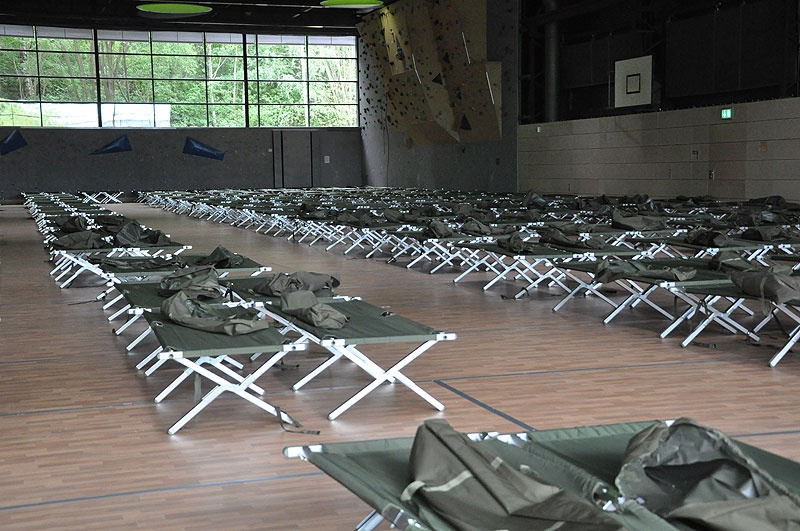
\includegraphics[width=.8\linewidth]{img/usz_feldbetten.jpg}
\caption*{\small \textit{Foto: Julia Vollmer, DNN-Online}}
\end{figure}